% Options for packages loaded elsewhere
\PassOptionsToPackage{unicode}{hyperref}
\PassOptionsToPackage{hyphens}{url}
%
\documentclass[
]{article}
\usepackage{amsmath,amssymb}
\usepackage{lmodern}
\usepackage{iftex}
\ifPDFTeX
  \usepackage[T1]{fontenc}
  \usepackage[utf8]{inputenc}
  \usepackage{textcomp} % provide euro and other symbols
\else % if luatex or xetex
  \usepackage{unicode-math}
  \defaultfontfeatures{Scale=MatchLowercase}
  \defaultfontfeatures[\rmfamily]{Ligatures=TeX,Scale=1}
\fi
% Use upquote if available, for straight quotes in verbatim environments
\IfFileExists{upquote.sty}{\usepackage{upquote}}{}
\IfFileExists{microtype.sty}{% use microtype if available
  \usepackage[]{microtype}
  \UseMicrotypeSet[protrusion]{basicmath} % disable protrusion for tt fonts
}{}
\makeatletter
\@ifundefined{KOMAClassName}{% if non-KOMA class
  \IfFileExists{parskip.sty}{%
    \usepackage{parskip}
  }{% else
    \setlength{\parindent}{0pt}
    \setlength{\parskip}{6pt plus 2pt minus 1pt}}
}{% if KOMA class
  \KOMAoptions{parskip=half}}
\makeatother
\usepackage{xcolor}
\usepackage[margin=1in]{geometry}
\usepackage{graphicx}
\makeatletter
\def\maxwidth{\ifdim\Gin@nat@width>\linewidth\linewidth\else\Gin@nat@width\fi}
\def\maxheight{\ifdim\Gin@nat@height>\textheight\textheight\else\Gin@nat@height\fi}
\makeatother
% Scale images if necessary, so that they will not overflow the page
% margins by default, and it is still possible to overwrite the defaults
% using explicit options in \includegraphics[width, height, ...]{}
\setkeys{Gin}{width=\maxwidth,height=\maxheight,keepaspectratio}
% Set default figure placement to htbp
\makeatletter
\def\fps@figure{htbp}
\makeatother
\setlength{\emergencystretch}{3em} % prevent overfull lines
\providecommand{\tightlist}{%
  \setlength{\itemsep}{0pt}\setlength{\parskip}{0pt}}
\setcounter{secnumdepth}{-\maxdimen} % remove section numbering
\usepackage{placeins}
\ifLuaTeX
  \usepackage{selnolig}  % disable illegal ligatures
\fi
\IfFileExists{bookmark.sty}{\usepackage{bookmark}}{\usepackage{hyperref}}
\IfFileExists{xurl.sty}{\usepackage{xurl}}{} % add URL line breaks if available
\urlstyle{same} % disable monospaced font for URLs
\hypersetup{
  pdftitle={BAM\_RAB v 0.1},
  pdfauthor={RFL, DTW, BPC},
  hidelinks,
  pdfcreator={LaTeX via pandoc}}

\title{BAM\_RAB v 0.1}
\author{RFL, DTW, BPC}
\date{2022-11-17}

\begin{document}
\maketitle

\hypertarget{preliminary-analyses}{%
\section{Preliminary Analyses}\label{preliminary-analyses}}

This document contains preliminary analyses regarding the BAM\_RAB data
set as it stands. These preliminary analyses focus on the following
elements: As,Cd,Cu,Fe,Pb,Se and Zn. These elements were selected based
on interest in the ``Big 5'' contaminants of concern plus Fe due to our
interest in particle formation. I also added Se given the current
interests of our extended research group, as well as some interesting
parallels between the behavior of Se and Zn.

\hypertarget{temporal-patterns-in-metal-accumulation-in-biomass-contents-mgg.}{%
\subsection{1. Temporal patterns in metal accumulation in biomass
contents
(mg/g).}\label{temporal-patterns-in-metal-accumulation-in-biomass-contents-mgg.}}

The following figures represent the patterns for all samples over time
within the three biomass compartments, all sites included. The code for
generation all these figures is located under
1\_code/2\_RFL\_Presentation\_Figures/1\_Barplots\_Time\_All.R

Arsenic (Fig.1) seems to be the only element that actually decreases
over time as the growing season progresses. I think this would be the
main suspect when we actually try to trace the relationship between
metals in algae and metals in water.

\begin{figure}
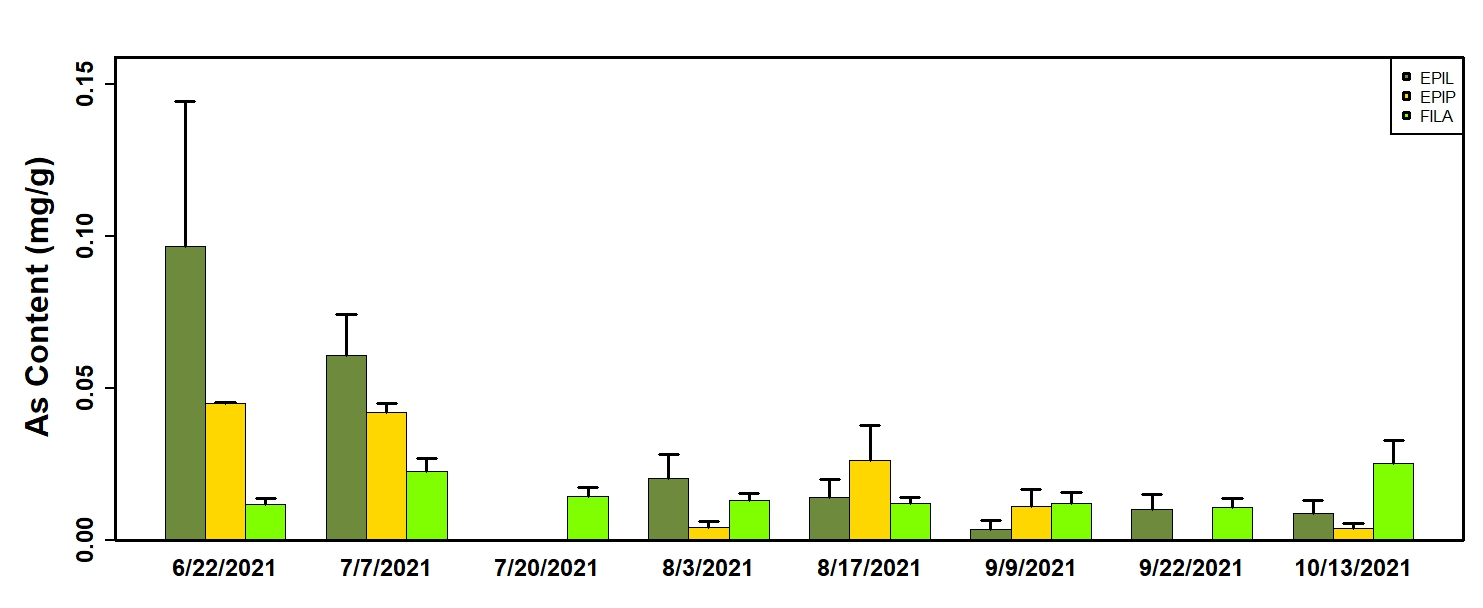
\includegraphics[width=1\linewidth]{Figures/1} \caption[Figure 1.1]{Figure 1.1: Arsenic content of benthic biomass compartments over time.}\label{fig:unnamed-chunk-1}
\end{figure}

\FloatBarrier

For most metals, patterns are pretty similar (Figs. 2,3,4,5).

\begin{figure}
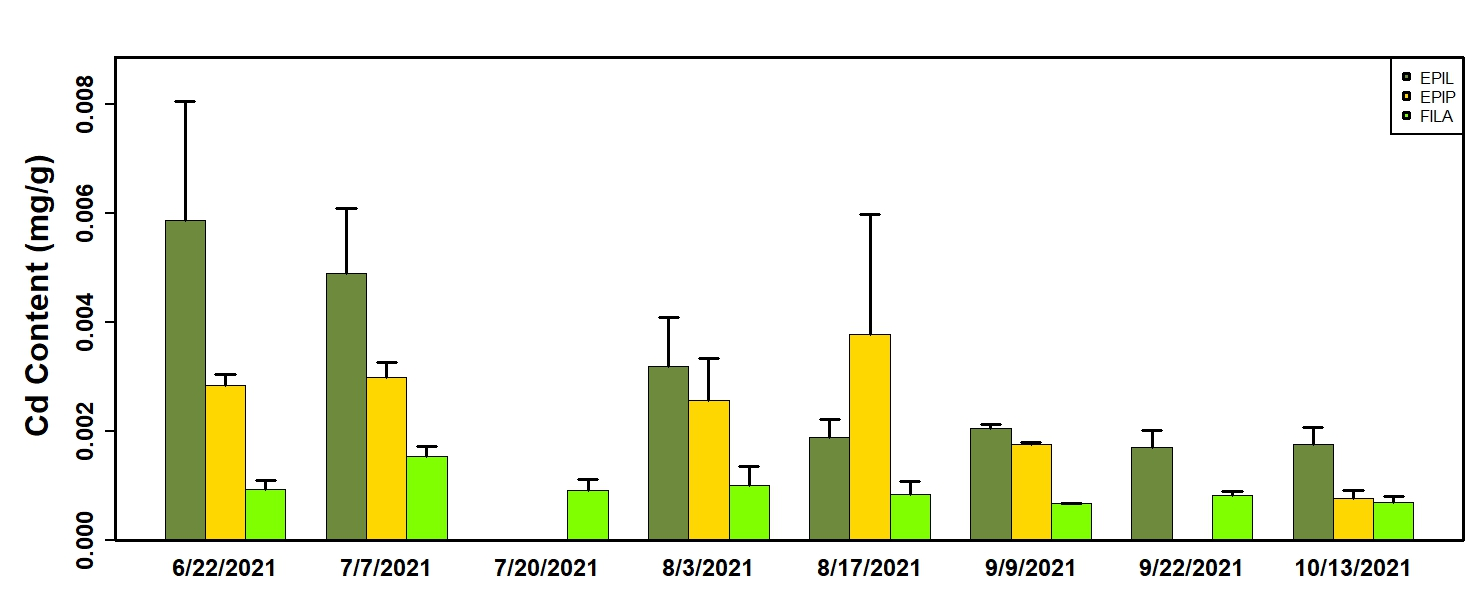
\includegraphics[width=1\linewidth]{Figures/2} \caption[Figure 1.2]{Figure 1.2: Cadmium content of benthic biomass compartments over time.}\label{fig:unnamed-chunk-2}
\end{figure}

\FloatBarrier

\begin{figure}
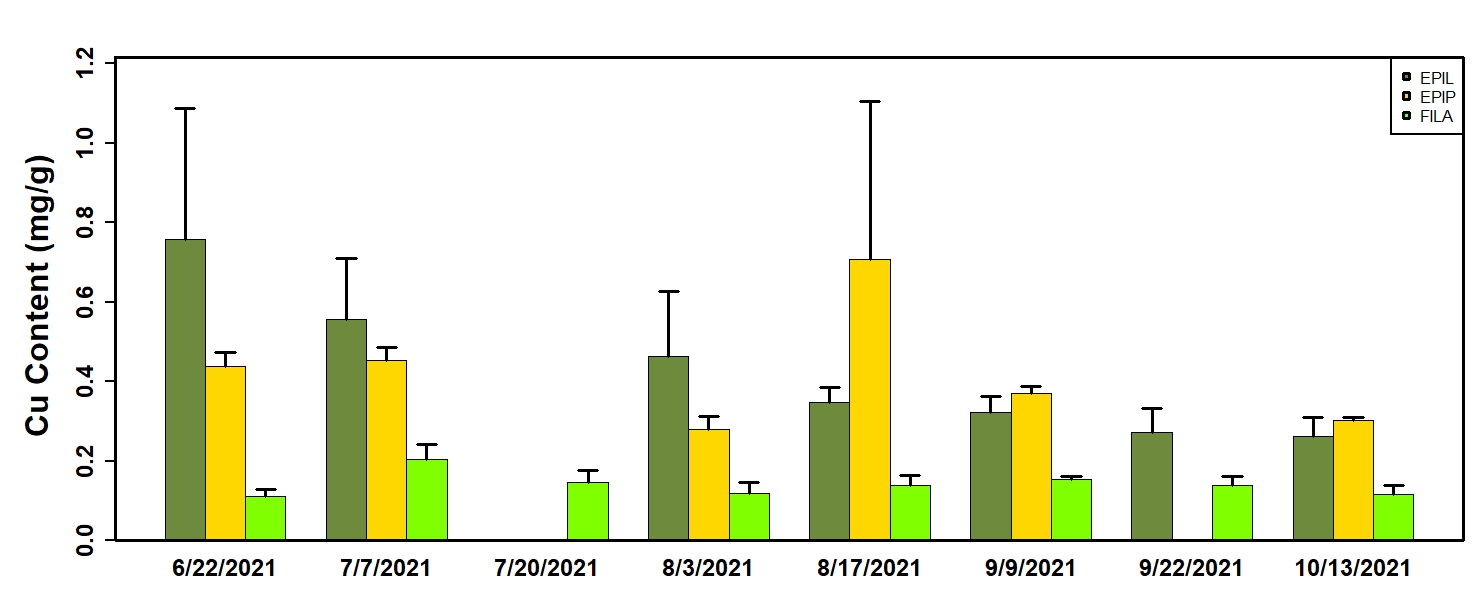
\includegraphics[width=1\linewidth]{Figures/3} \caption[Figure 1.3]{Figure 1.3: Copper content of benthic biomass compartments over time.}\label{fig:unnamed-chunk-3}
\end{figure}

\FloatBarrier

\begin{figure}
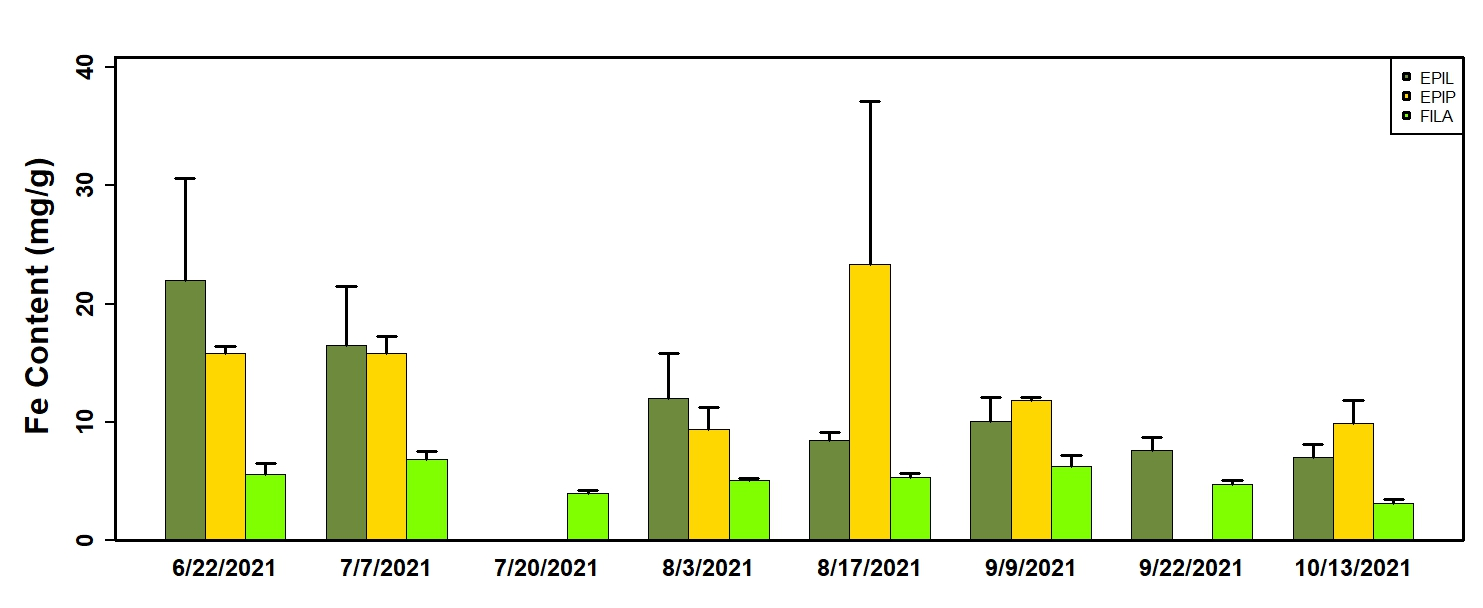
\includegraphics[width=1\linewidth]{Figures/4} \caption[Figure 1.4]{Figure 1.4: Iron content of benthic biomass compartments over time.}\label{fig:unnamed-chunk-4}
\end{figure}

\FloatBarrier

\begin{figure}
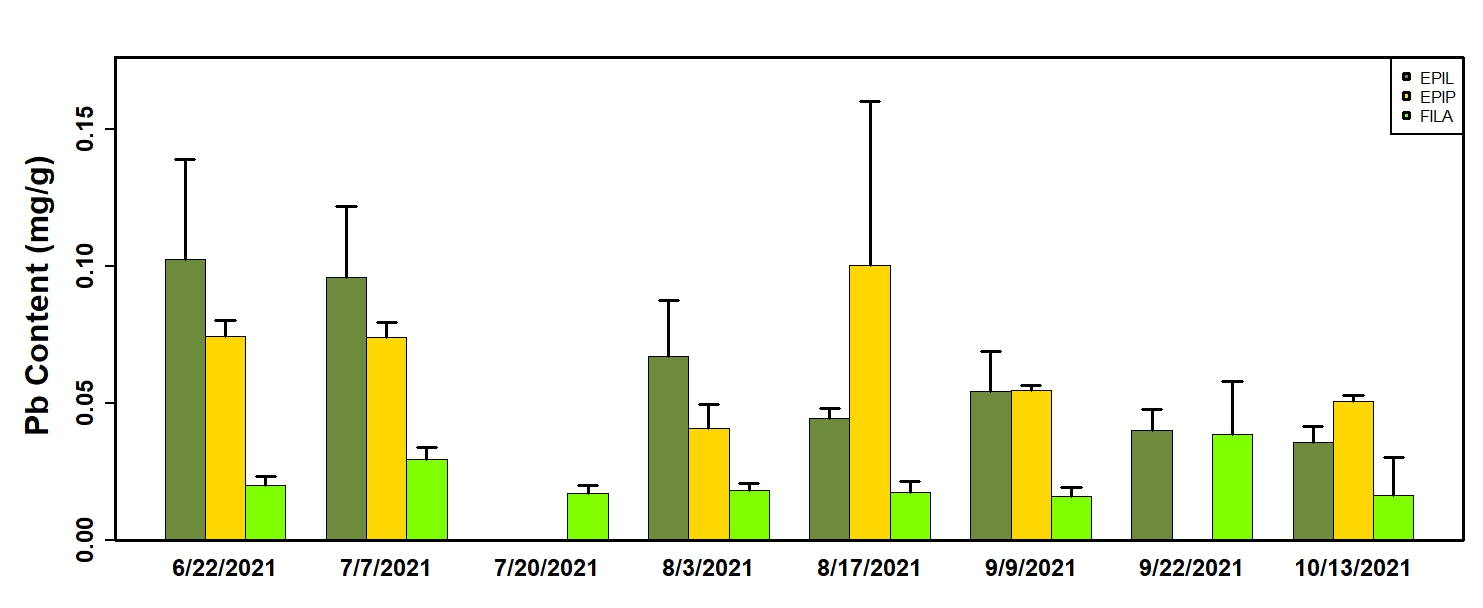
\includegraphics[width=1\linewidth]{Figures/5} \caption[Figure 1.5]{Figure 1.5: Lead content of benthic biomass compartments over time.}\label{fig:unnamed-chunk-5}
\end{figure}

\FloatBarrier

\newpage

Now we we get to the 2 elements that actually differ. Selenium seems to
peak earlier in the season (when compared to Cd,Cu, Fe and Pb).

\begin{figure}
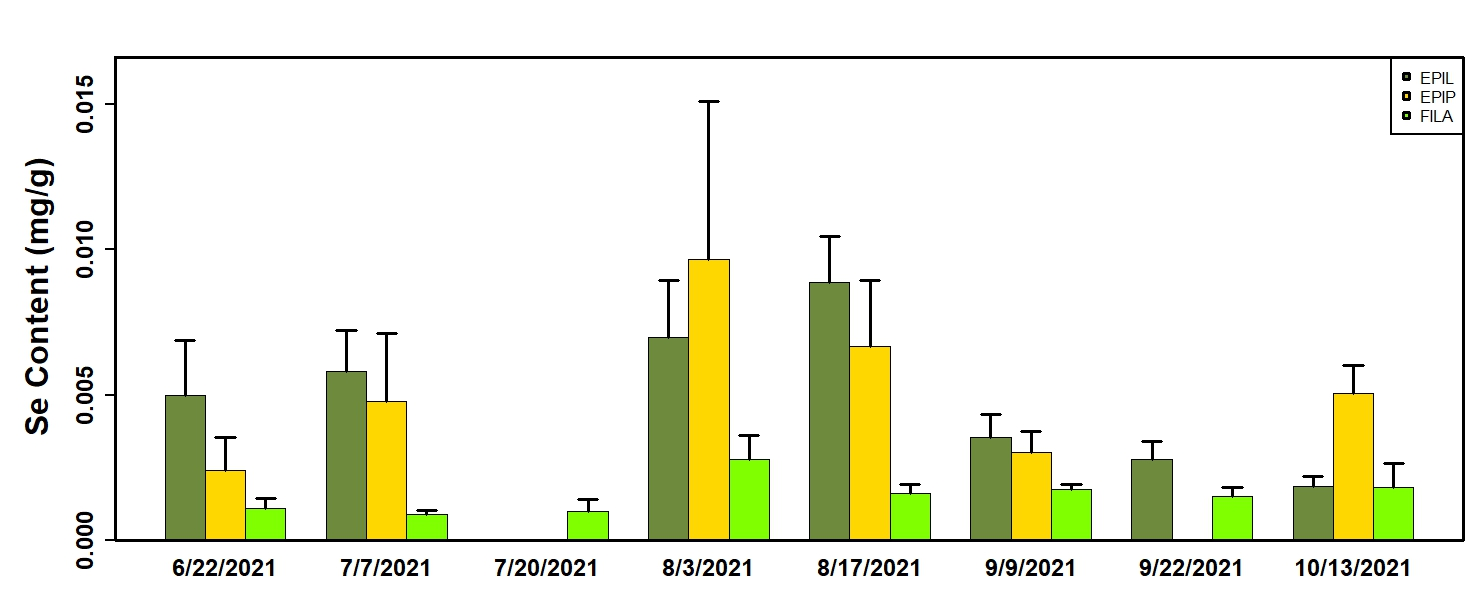
\includegraphics[width=1\linewidth]{Figures/6} \caption[Figure 1.6]{Figure 1.6: Selenium content of benthic biomass compartments over time.}\label{fig:unnamed-chunk-6}
\end{figure}

\FloatBarrier

And of course, as discussed before, Zn is not really present in
filamentous algae. Looking at the other compartments it does not seem to
present any temporal trends.

\begin{figure}
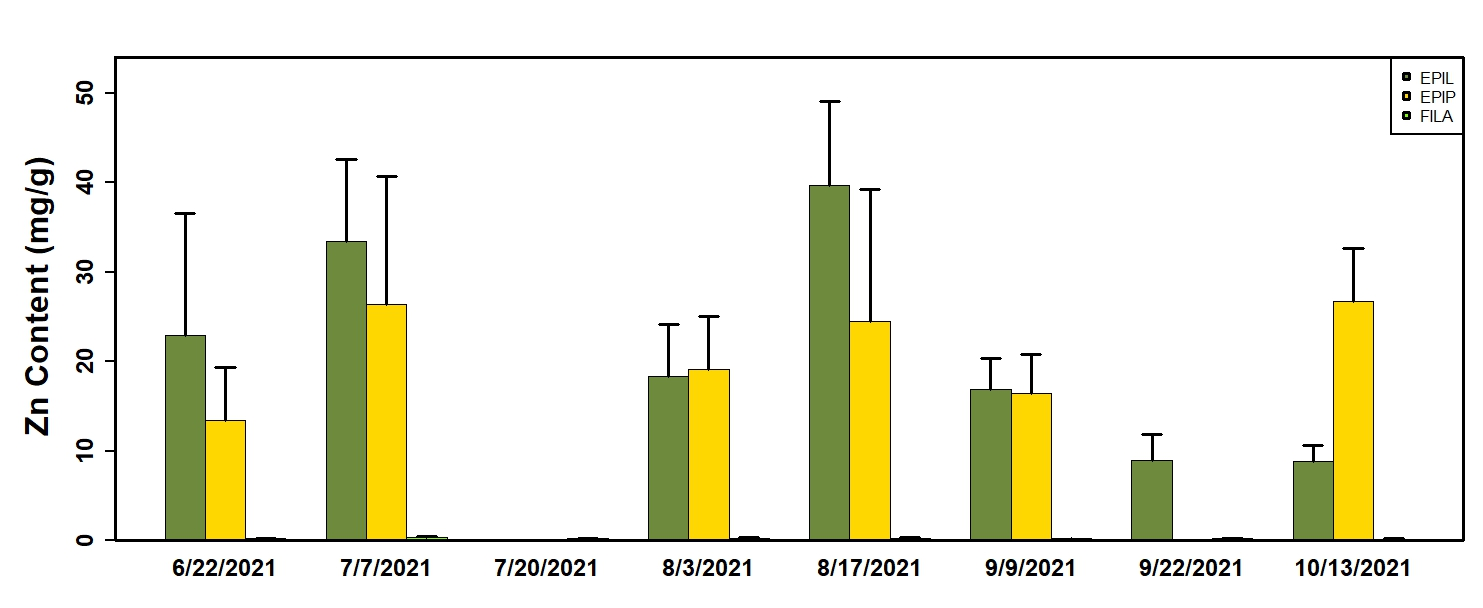
\includegraphics[width=1\linewidth]{Figures/7} \caption[Figure 1.7]{Figure 1.7: Zinc content of benthic biomass compartments over time.}\label{fig:unnamed-chunk-7}
\end{figure}

\FloatBarrier

\newpage

\hypertarget{temporal-patterns-in-metal-stocks-for-individual-sites.}{%
\subsection{2.Temporal patterns in metal ``stocks'' for individual
sites.}\label{temporal-patterns-in-metal-stocks-for-individual-sites.}}

\newpage

\hypertarget{correlation-between-metals-among-compartments}{%
\subsection{Correlation between metals among
compartments}\label{correlation-between-metals-among-compartments}}

\newpage

\hypertarget{principal-component-analyses-of-contents-and-stocks-by-compartment.}{%
\subsection{Principal component analyses of contents and stocks by
compartment.}\label{principal-component-analyses-of-contents-and-stocks-by-compartment.}}

PCA analysis was performed in a two tier fashion. Firstly, I performed a
PCA analysis on all samples using the BIG5+ elements (As,Cd,Cu,Fe,Pb,Se
and Zn) for both metal contents (mg/g) and stocks (mg/m2). However, due
to the high collinearity (next figure, still figuring out figure
numbering in Markdown) I performed a Variance Inflation test to
eliminate highly collinear variables and retain the elements that
comprise the highest amount of variance. I did this independently for
contents and stocks.I'm calling this group of variables ``LEASTVIF''.

\begin{figure}
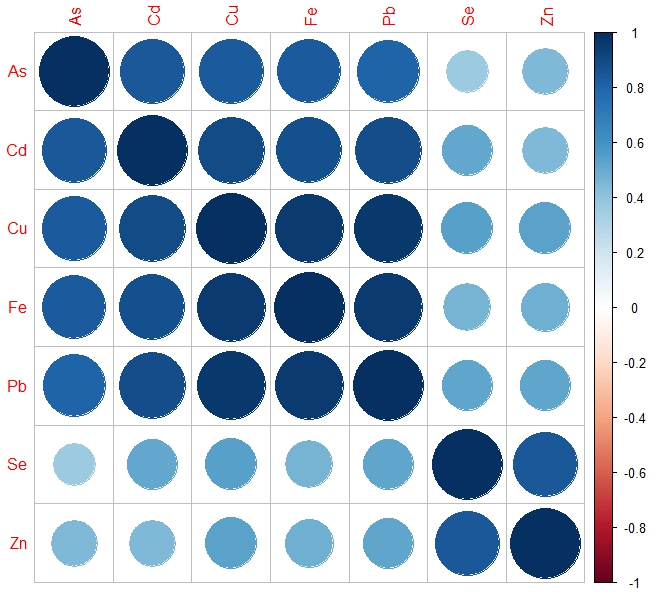
\includegraphics[width=1\linewidth]{Figures/CORRPLOT_1_BIG5PLUS} \caption[Correlation plots of BIG5+ elemental contents for all biomass compartments combined]{Correlation plots of BIG5+ elemental contents for all biomass compartments combined.}\label{fig:unnamed-chunk-8}
\end{figure}

\FloatBarrier

\newpage

These are the PCA results for contents using the BIG5+ elements.
Variables have been logged, scaled and centered.

\begin{figure}
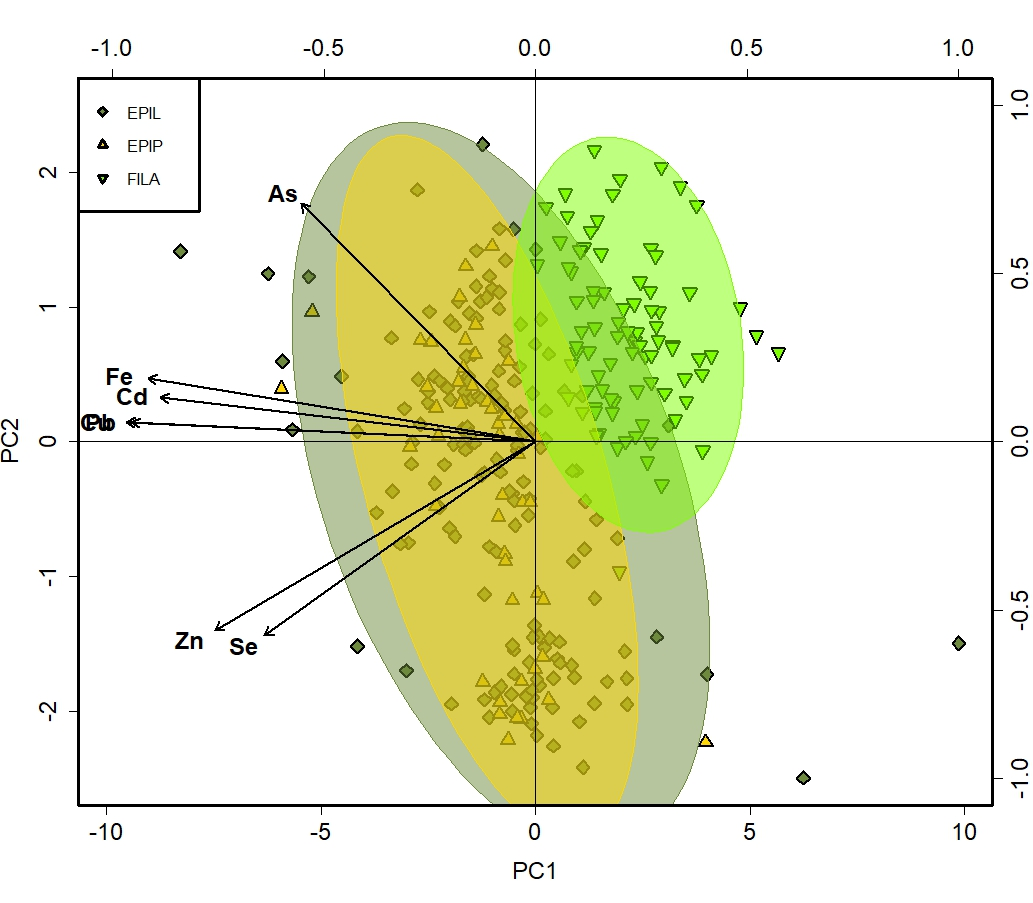
\includegraphics[width=1\linewidth]{Figures/PCA_1_BIG5PLUS} \caption[Prinicipal component analysis of BIG5+ elemental contents for three different biomass compartments]{Prinicipal component analysis of BIG5+ elemental contents for three different biomass compartments. Secondary X and Y axes (top and right) indicate correlation between variables and principal components.}\label{fig:unnamed-chunk-9}
\end{figure}

\FloatBarrier

\newpage

Here is the correlation plot for the LEASTVIF contents dataset.
Variables retained were Be,Ca,Co,Mo,Pb,S,Se,Si and Sn.

\begin{figure}
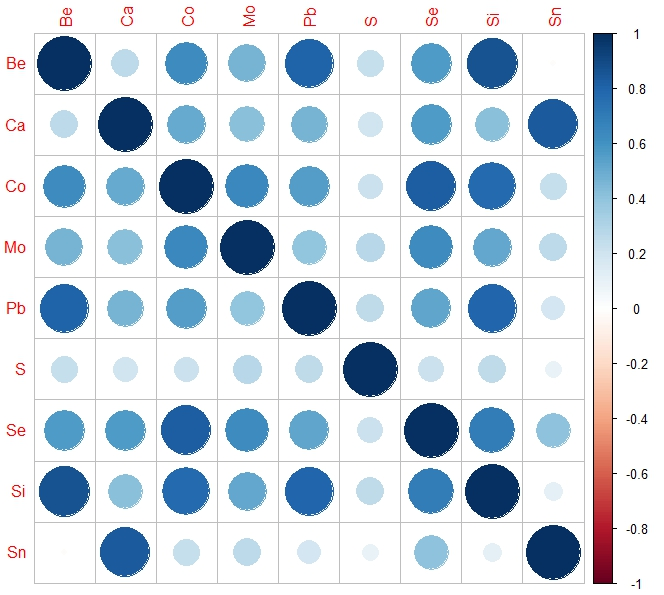
\includegraphics[width=1\linewidth]{Figures/CORRPLOT_1_LEAST_VIF} \caption[Correlation plots of LEASTVIF elemental contents for all biomass compartments combined]{Correlation plots of LEASTVIF elemental contents for all biomass compartments combined.}\label{fig:unnamed-chunk-10}
\end{figure}

\FloatBarrier

These are the results for contents using the LEASTVIF elements.
Variables have been logged, scaled and centered.

\newpage

\begin{figure}
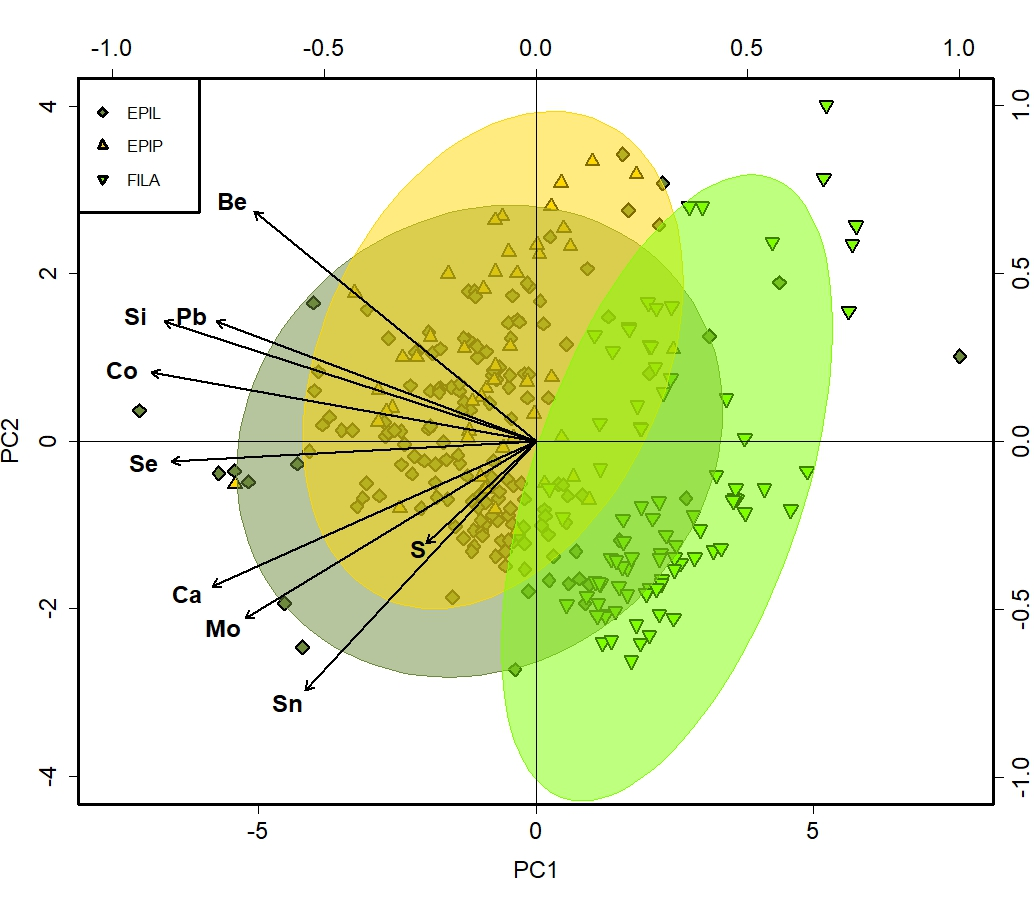
\includegraphics[width=1\linewidth]{Figures/PCA_1_LEASTVIF} \caption[Prinicipal component analysis of LEASTVIF elemental contents for three different biomass compartments]{Prinicipal component analysis of LEASTVIF elemental contents for three different biomass compartments. Secondary X and Y axes (top and right) indicate correlation between variables and principal components.}\label{fig:unnamed-chunk-11}
\end{figure}

\FloatBarrier

\newpage

Here are the results for stocks for BIG5 and LEASTVIF:

\begin{figure}
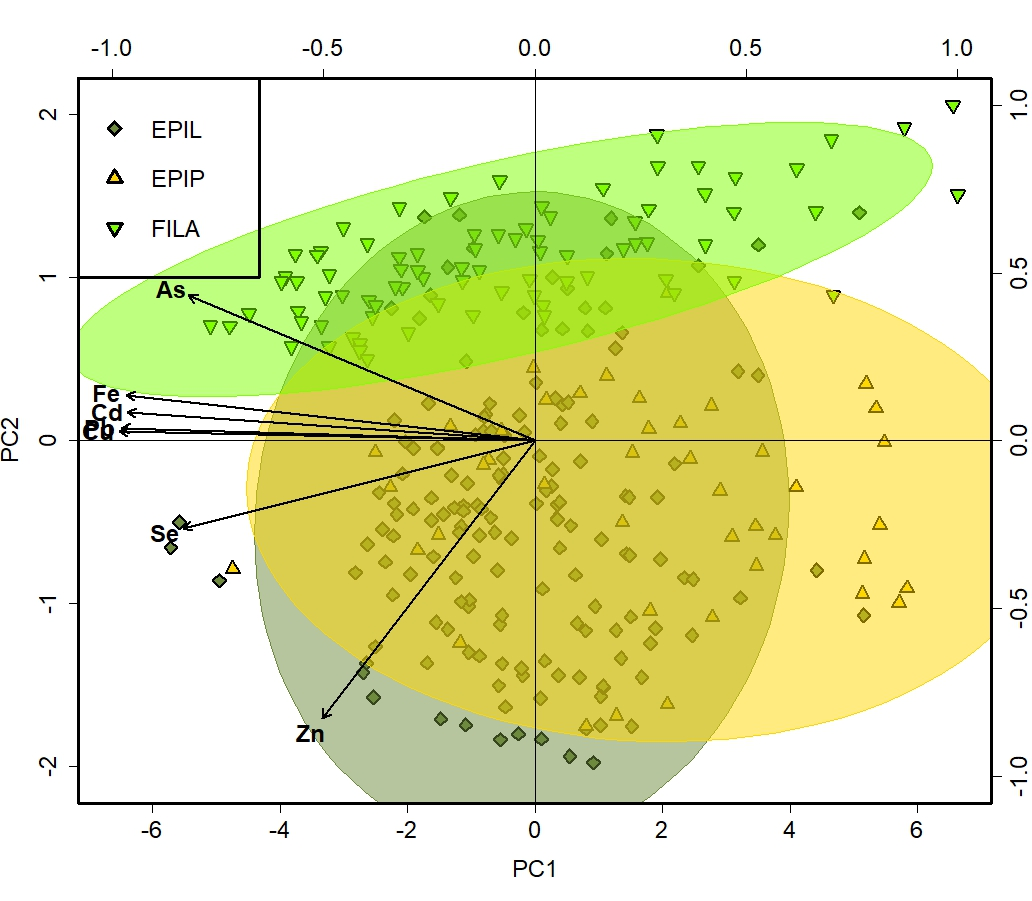
\includegraphics[width=1\linewidth]{Figures/PCA_2_BIG5PLUS} \caption[Prinicipal component analysis of BIG5+ elemental stocks for three different biomass compartments]{Prinicipal component analysis of BIG5+ elemental stocks for three different biomass compartments. Secondary X and Y axes (top and right) indicate correlation between variables and principal components.}\label{fig:unnamed-chunk-12}
\end{figure}

\FloatBarrier

\begin{figure}
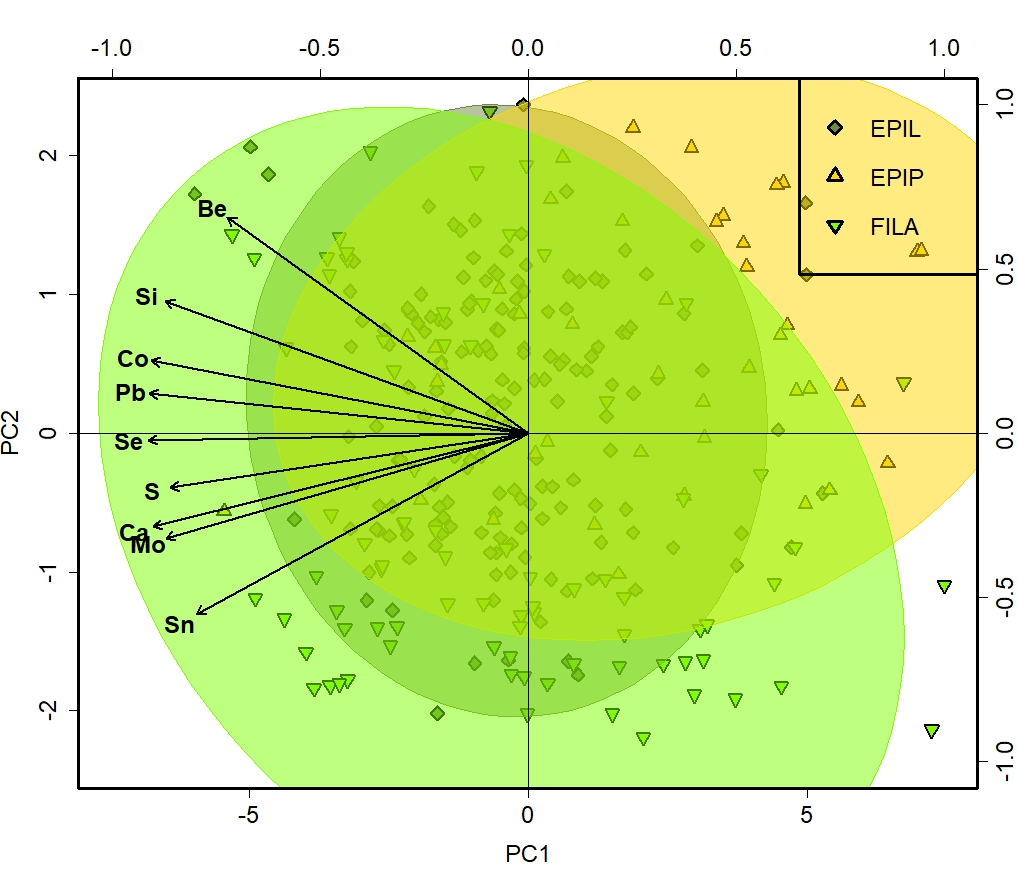
\includegraphics[width=1\linewidth]{Figures/PCA_2_LEASTVIF} \caption[Prinicipal component analysis of LEASTVIF elemental stocks for three different biomass compartments]{Prinicipal component analysis of LEASTVIF elemental stocks for three different biomass compartments. Secondary X and Y axes (top and right) indicate correlation between variables and principal components.}\label{fig:unnamed-chunk-13}
\end{figure}

\FloatBarrier

\newpage

Next steps are to extract PCA scores for samples and see how they vary
with time and pigment contents.

\hypertarget{methods}{%
\subsection{Methods}\label{methods}}

\#\#Study area

\#\#Field Sampling

\#\#\#Biomass

\#\#\#Water

\#\#Biomass sample processing

\#\#Nutrient Analysis

\#\#Metal Analysis

\#\#Metabolic measurements

\#\#Other?

\hypertarget{results}{%
\section{Results}\label{results}}

\hypertarget{discussion}{%
\section{Discussion}\label{discussion}}

\end{document}
